% 
%  chapter1.tex
%  ThesisISEL
%  
%  Created by Serge Lage on 2019/07/30.
%
% ================
% = Data =
% ================
\chapter{Data}
\label{cha:data}
This chapter provides the information about the used data and some analysis on it in how to use it for my work.

\section{VMS Records} % (fold)
\label{sec:vms_records}

VMS Data provided by the Xsealence enterprise contained data generated by the MONICAP “Blue Box”. Information about the localization, direction and velocity of the vessel at each 10 minutes, is saved in a local database. VMS datasets contained a vessel identification code, a timestamp, the latitude and longitude positions, the speed and direction. In this dataset there are 537138 entries from thirty vessels. These data is from vessels operating in the Portuguese shore.  
This dataset is created automatically by the MONICAP system and follows the concept of integrity and confidentiality.\\
The variables registered in the dataset are:
\begin{itemize}
\item VesselID: Vessel identification;
\item	Utc: Date time of the log;
\item	Gps \textemdash id: identification of the GPS in use (0 = GPS with EGNOS, 1 = MiniCs GPS);
\item	Fix/fix2: types of fix in the GPS:
\begin{itemize}
\item	0 = invalid, 
\item	1 = standard: valid, without integrity (without EGNOS), 
\item	2 = differential: valid, with integrity (with EGNOS), 
\item	3 = integrity: valid with integrity (with EGNOS);
\end{itemize}
\item	Lat/Lat2: latitude of GPS primary/secondary (in decimal);
\item	Lon/Lon2: longitude of GPS primary/secondary (in decimal);
\item	Cog: Course Over Ground. Varies from 0 to 360 clockwise, being 0, facing north;
\item	Sog: Speed Over Ground (velocity in knots);


\end{itemize}


In Table \ref{table:vms_records} we can see the summary of the data used in this project. The number of occurrences is 769928. 
Some cells of the table are with \textit{\-} because its not applicable for qualitative data.
The \textit{Quar} stands for Quartile and \textit{SD} stands for Standard deviation.

\begin {table}[h]
\small
\begin{center}
\begin{tabular}{c|c|c|c|c|c|c|c}
             & Minimum & Maximum & Average & 1 \textsuperscript{st} Quar & Median &  3\textsuperscript{rd} Quar & SD\\
\hline
Lon     & -52.706 & 35.965 & -4.493 &-9.811&-9.115&-7.986&21.156\\
Lat         & -35.243 &76.064&25.933&33.038&38.423&40.21&25.916\\
Sog         &  0 &42&4.183&1.634&3.012&7.399&3.211\\
Cog        &   0&360&166.31&68.89&173.125&255.69&108.64\\
utc        &  \begin{tabular}{@{}c@{}} 2008-10-30 \\ 21:50:58\end{tabular} &-&-&-&-&-\\
gps\_ id        & 0&1&-&-&-&-&-\\
fix        &   1&3&-&-&-&-&-\\
Fix2       &  0&2&-&-&-&-&-\\
Lon2        &   -52.706&155.977&-3.702&-9.726&-8.991&0&20.933\\
Lat2         &   -35.24&76.064&23.663&0&37.595&40.191&26.383\\
VesselId        & 1&38&-&-&-&-&-
           
\label{table:vms_records}
\end{tabular}
\caption {VMS Records}
\end{center}
\end {table}


% section vms_records (end)
\newpage 


\section{VMS Vessels} % (fold)
\label{sub:vms_vessels}
VMS Vessels is the vessel information that goes along with the VMS Records. These data contain information about vessels and fishing activities for which they are licensed.  \\
The variables registered in the dataset are:
\begin{itemize}
\item	ID: Vessel identification (VesselID/VMSRecords, foreign key);
\item	Name: Name of the vessel;
\item	Loa: Length Overall; 
\item	GT: Gross Tonnage;
\item	HP: Vessel power (HP);
\item	kW: Vessel power (KW);
\item	License: Registration of the vessel's licenses;
\item	PriGearCode: FOA code of the principal fishery device;
\item	SecGearCode: FOA code of the secondary fishery device.
\end{itemize}
%In Appendix A a detailed descriptive analysis of these variables is provided.

In Table \ref{table:vms_vessels} we can see the summary of the data regarding the vessels in the table VMS Records. This data was filtered from 56 occurrences to 38. The deleted data was referred to Vessels that haven’t data in the table VMS Records, so this vessels information’s was superfluous to ours needs. In Appendix \ref{appendix:anexo1} we discriminate the fishing licenses. 


\begin {table}[H]
\small
\begin{center}
\begin{tabular}{c|c|c|c|c|c|c|c}
            &  Minimum & Maximum & Average & 1 \textsuperscript{st} Quar & Median & 3\textsuperscript{rd} Quar & SD \\
\hline
ID     & 1&38&-&-&-&-&-\\
Name         &-&-&-&-&-&-&-\\
Loa         & 11.95&84.94&23.48&16.93&19.35&23.70&15.49\\
GT        &22251&18.99&200.28&27.98&57.15&110.34&473.78\\
HP        & 3600&130&539&230&350&497&689.56\\
KW        &2684.50&95.62&396.52&172.84&259.21&367.91&498.54\\
License        &-&-&-&-&-&-&-\\
PriGC       &-&-&-&-&-&-&-\\
SecGC        &-&-&-&-&-&-&-


           
\label{table:vms_vessels}
\end{tabular}
\caption {VMS Vessels}
\end{center}
\end {table}

% section vms_vessels (end)


\section{Data Analysis} % (fold)
\label{sub:data_analysis}



The data used as input to the models is VMS Records data. Within which the speed and location data are the ones that could have some demarking between the types of fishing.\\
About the locations, certain fishing types only ocourre in certain depth. So the locations can help in this cases. \\
In order to meet the objectives we need to understand the velocity patterns.
The first feature we find when studying speed is its separation into two distributions.

\begin{figure}[h]
    \centering
    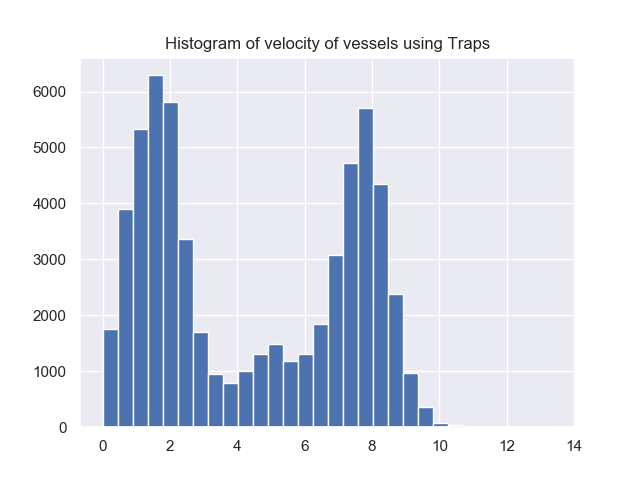
\includegraphics[width=0.8\linewidth]{Chapters/img/h_armadilhas.png}
    \caption{Histogram of velocity of traps license.}
    \label{fig:h_armadilhas}
\end{figure}

%\begin{figure}[h]
%    \centering
%    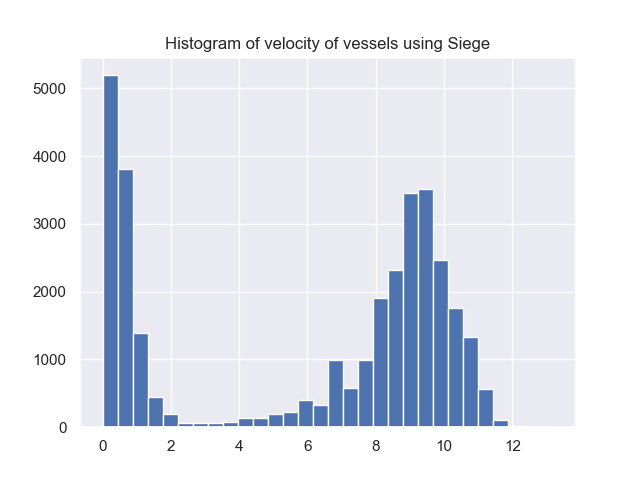
\includegraphics[width=0.8\linewidth]{Chapters/img/h_cerco.png}
%    \caption{Histogram of velocity of siege license.}
%    \label{fig:h_cerco}
%\end{figure}

\begin{figure}[h]
    \centering
    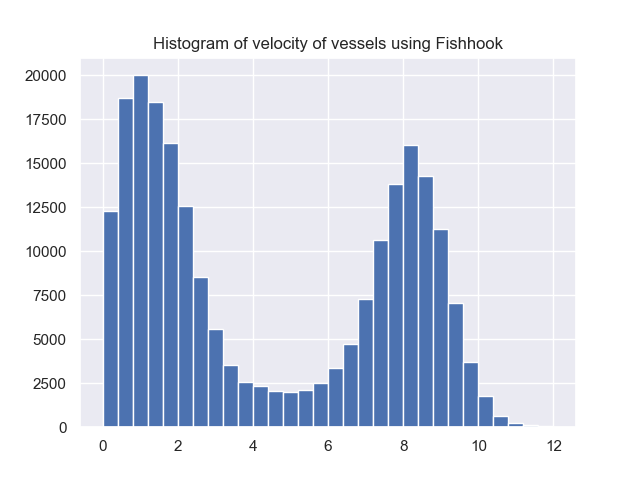
\includegraphics[width=0.8\linewidth]{Chapters/img/h_linha.png}
    \caption{Histogram of velocity of fishhook license.}
    \label{fig:h_linha}
\end{figure}

As we can see in Figure \ref{fig:h_armadilhas} that at lower speeds we have the speeds at which the vessel is fishing and the higher speeds represent the movements of the vessel from the port to the fishing grounds and back to the port.





Knowing this we can notice that different types of fishing have different fishing speeds as we can see the differences between the histogram in Figure \ref{fig:h_armadilhas} containing data on fishing vessels using traps and Figure \ref{fig:h_linha} concerning fishing vessels using fishhook.





It is important to separate the inputs representing fishing speeds from the others in the data as the input to the models used in Chapter 5 it is necessary to have the data filtered out only with the fishing activity data.
Data from other operations that are not fishing must be discarded because there are not discriminatory for the fishing type. For example, speed 0 nautical miles is not interesting as all vessels, regardless of their type of fishing, stop at the fishing port.
Hence the importance of Chapter 4.


% section data_analysis (end)

% chapter data (end)



